\documentclass[12pt]{article}
\usepackage{amssymb, amsthm, graphics, graphicx}
\usepackage{amsmath}
\usepackage{url}

%these are initial settings. Ron recommended them, so that's just what I use.
\textwidth = 6.5 in
\textheight = 9 in
\oddsidemargin = 0.0 in
\evensidemargin = 0.0 in
\topmargin = -.75in
\parskip = 0.2 in
\parindent = 15 pt
\renewcommand{\baselinestretch}{1.25}
\renewcommand*{\thefootnote}{[\arabic{footnote}]} %square brackets

\providecommand{\e}[1]{\ensuremath{\times 10^{#1}}}
\providecommand{\degree}[0]{\ensuremath{^{\circ}}}

\providecommand{\ah}[1]{\ensuremath{\hat{a}_{#1}}}
\providecommand{\ahx}[0]{\ensuremath{\ah{x}}}
\providecommand{\ahy}[0]{\ensuremath{\ah{y}}}
\providecommand{\ahz}[0]{\ensuremath{\ah{z}}}
\providecommand{\pfs}[0]{\ensuremath{\epsilon_{0}}} %permittivity of free space => 1/(36\pi) \e{-9}
%\providecommand{\vec}[1]{\ensuremath{\textbf{#1}}} %vector notation ACTUALLY \vec is _real_ vector notation
\providecommand{\ohm}[0]{\ensuremath{\Omega}}


\newtheorem*{prob}{Problem}

\begin{document}
\begin{flushright}
\textbf{Charles Julian Knight}\\
ECE4892\\
\today
\end{flushright}


\begin{center}
\huge HW 1
\end{center}

\begin{prob}[1.a]{
  Design an circuit with a single op amp that will covert pitch control voltages from the Moog standard to the Buchla standard. You may assume that your conversion module is given an input from a voltage source with zero output impedance and is being fed to a module with an infinite input impedance; you also do not need to worry about input and output protection (assume nobody will be abusing your module). For this part of the exercise, assume you have perfect ``zero-tolerance'' resistors.
}\end{prob}

Since the Moog standard is lower than the Buchla standard and we don't want to invert the signal, let's use
a non-inverting amplifier with a gain of
\[ \frac{V_o}{V_i} = \frac{1.2V}{1V} = 1.2 = \left(1+\frac{R_i}{R_f}\right) \rightarrow R_i = .2R_f \]
If we pick $R_i = 1k\ohm$, then $R_f = 20k\ohm$, both of which are common resistor values.

\begin{prob}[1.b]{
  Off-the-shelf resistors never exactly match their listed values. Let's do a ``worst case'' analysis for the case where your circuit is given a one volt input. If you use 5\% resistors, assuming the true resistance is uniformly distributed, what is the highest voltage you might get out? What is the lowest voltage? How many semitones above and below the desired value are these voltages in the Buchla pitch standard?
}\end{prob}

The highest gain would happen when $R_i$ is $5\%$ too big and $R_f$ is $5\%$ too small (and vice versa for the lowest gain). 
\[ 1V \left(1+\frac{1.05R_i}{.95R_f}\right) = 1.221V \rightarrow +0.21 semitones \]
\[ 1V \left(1+\frac{.95R_i}{1.05R_f}\right) = 1.181V \rightarrow -0.19 semitones \]

This means the notes would be about $20$ cents sharp or flat. 

\begin{prob}[1.c]{
  Repeat the above analysis for 1\% resistors.
}\end{prob}

\[ 1V \left(1+\frac{1.01R_i}{.99R_f}\right) = 1.204V \rightarrow +0.04 semitones \]
\[ 1V \left(1+\frac{.99R_i}{1.01R_f}\right) = 1.196V \rightarrow -0.04 semitones \]

This means the notes would still be about $4$ cents sharp or flat. According to a Georgia Tech student's master's thesis\footnote{\url{https://en.wikipedia.org/wiki/Cent_(music)#Human_perception}}, the limits of human pitch perception are around $5-6$ cents, so you could probably get away with these resistors.
%%%%%%%%%%%%%%%%%%%%%%%%%%%%%%%%%%%%%%%%%%%%%%%%%%%%%%%%%%%%%%%%%%%%%%%%%%%%%%%%%%%%%%%%%%%%%%%%%%%%%%%%%%

\begin{prob}[2.a]{
  Find the voltage at the output of IC3:B. You can do this quickly if you realize that this op amp is acting in a standard ``inverting mixer'' configuration. (Remember we are assuming the wiper of the ``pan'' pot is at ground).
}\end{prob}
This opamp appears to be in an inverting setup. By our ideal opamp rules, the inverting pin must be a virtual ground. Since the pan pot is also at ground, no current flows through R7. Thus the current through R3 is $\frac{V^- - 0}{120k} = -.1mA$. That same current flows through R5, so the output voltage must be
\[0.1mA *100k\ohm = 10V\footnote{Or simply $-12*-100k/120k=10$}\]

\begin{prob}[2.b]{
  Given all the notes above and the assumption that the current through the base of Q2 is negligible, so we may approximate its collector and emitter currents as being equal, find the current input to the OTA ($I_{con}$) as a function of $V_{con}$.
}\end{prob}
Since the inverting input of the opamp is at virtual ground, there's a current comming from IC3B of $10V/100k=.1mA$ and a current coming from our control J5 $V_{con}/100k$. Some of those two currents are going to $V^-$ through R16, but the rest must be going through R12. The current through R12 (let's call it $I_{12}$) must be $I_{12}=.1mA + V_{con}/100k - .0545mA =.04545mA -V_{con}/100k$. That means the voltage at the emitter of Q2 is $-10K I_{12}$. So $I_{con}$ is $I_{12}$ plus the part that goes through R18 from ground. So in total,
\[I_{con} = I_{12} + I_{12}\frac{10k}{1.5k} = 7.66I_{12} = .349mA - \frac{7.66V_{con}}{100k} \]
%  R12 and R18 appear to be in parallel. Thus
% \[I_{con} = \frac{V_{con}}{R12||R18} = \frac{V_{con}}{1.3K\ohm} \]

\begin{prob}[2.c]{
  Now let's look at the main part of the VCA, with input at J2 and output at J11. Find the gain of the VCA as a function of $I_{con}$. For now, you may ignore C12 (i.e. open the cap, which is a reasonable assumption for low frequencies).
}\end{prob}
We're taking the non-inverting input of the 13600 to be ground. I'll call the signal at J2 $V_{in}$ and at J11 $V_{out}$. We know the output of the OTA to be
\[I_{out} = I_{con}\frac{\left(\frac{220}{220+22k}\right)V_{in} -0}{2V_T}\]
Then $I_{out}$ is fed into an inverting amp. If that same current is through R52, then $V_{out} = R52 I_{out}$. The gain is then
\[ 33k\frac{\left(\frac{220}{220+22k}\right)}{2V_T}I_{con} = -(6.283 mA^{-1})I_{con} \]

\begin{prob}[2.d]{
  Suppose $V_{con}$ = 10V (from what I understand, the envelope generators in the PAiA 9700 series can generate up to 10V, so that's a reasonable voltage to try). What is $I_{con}$ in this case?
}\end{prob}
Assuming my equation in part b is correct,
  \[ I_{con} = 7.66I_{12} = .349mA - \frac{7.66\cdot10V}{100k} = -.417 mA \]

\begin{prob}[2.e]{
  Take a look at the ``Absolute Maximum Ratings'' section of the LM 13600 datasheet. What is the maximum rating for the control current (which the data sheet will call $I_{ABC}$)? Is the value you found in part (d) above or below this?
}\end{prob}
The max current is $2mA$, so this is quite a safe current.

\begin{prob}[2.f]{
  What is the gain of the VCA for $V_{con}$ = 10 V?
}\end{prob}
Assuming my equation for part c is correct,
\[A = -(6.283 mA^{-1})I_{con} = 2.62347 \]

\begin{prob}[2.g]{
  Without going through extensive calculations - i.e., by just reasoning your way through the circuit - what happens to the VCA gain as the wiper of the ``pan'' pot is turned away from ground and toward V+.
}\end{prob}
Sweeping the pan pot decreases $I_{con}$ for the right VCA that we were analyzing which reduces the gain, but at the same it increases $I_{con}$ for the left VCA which has an identical circuit amplifying J1 to J10.

\begin{prob}[2.h]{
  Previously, we ignored C12. If we now consider it, we see that C12, R52, and IC6:B act as a current-to-voltage single-pole lowpass filter with a cutoff frequency (half-power point) of $1/(2\pi RC)$). What is the cutoff frequency of this filter? Is this cutoff frequency above or below the limit of typical human hearing?
}\end{prob}
\[f_c = \frac{1}{2\pi RC} = 48.2 KHz\]
which is much higher than 20 KHz. I imagine this helps avoid high-frequency oscillations.

\begin{prob}[2.i]{
  What is the input impedance of the VCA?
}\end{prob}
Looking in from J2, the signal sees a $22K\ohm$ and $220\ohm$ series resistance to ground. So the input impedance is $22.22k\ohm$.

\begin{prob}[2.j]{
  What is the output impedance of the VCA? (Assume the op amps are all ideal, i.e., they have zero output impedance).
}\end{prob}
At J10 and J11, they didn't put any series output resistors, so it is theoretically (not practically) infinite. But on J12, which could be some sort of mixdown of left and right, the output impedance is R116$||$R117 = $5k\ohm$.

% %%%%%%%%%%%%%%%%%%%%%%%%%%%%%%%%%%%%%%%%%%%%%%%%%%%%%%%%%%%%%%%%%%%%%%%%%%%%%%%%%%%%%%%%%%%%%%%%%%%%%%%%%%%5
\begin{prob}[3]{
  On a single graph, plot (a) the voltage at ``C'' as a function of R, for $0 < R < 10K$, and (b) the same thing as (a), except suppose that the 120K resistor is actually a 10K resistor. I recommend using MATLAB to make the graph, but you may use whatever computer program you prefer.\\ Which graph, (a) or (b), looks more linear?
}\end{prob}
\[V_{out}(R) = V^+ \left(\frac{(R||120k)}{(R||120k)+(10k-R)}\right)\]
\begin{verbatim}
EDU>> R = linspace(1,10000);
EDU>> R2=120000;
EDU>> V=12;
EDU>> parallel = (R*R2)./(R+R2);
EDU>> out = V*(parallel./(parallel + (10000-R)));
EDU>> plot(R, out)
EDU>> R2=10000;
EDU>> parallel = (R*R2)./(R+R2);
EDU>> out = V*(parallel./(parallel + (10000-R)));
EDU>> plot(R, out)
\end{verbatim}
\begin{center}
  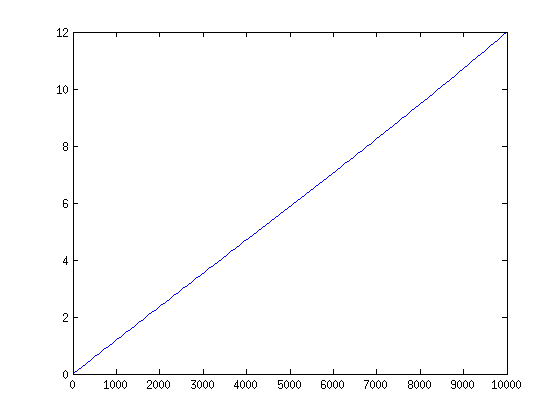
\includegraphics[width=3in]{r2is120k.png}
  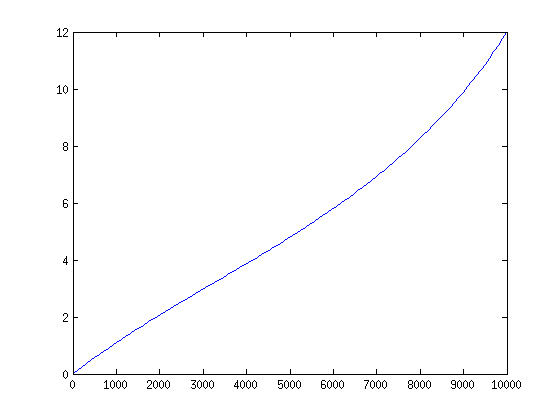
\includegraphics[width=3in]{r2is10k.png}
\end{center}
I think it is pretty obvious why R7 is $>>$ R109.

% %%%%%%%%%%%%%%%%%%%%%%%%%%%%%%%%%%%%%%%%%%%%%%%%%%%%%%%%%%%%%%%%%%%%%%%%%%%%%%%%%%%%%%%%%%%%%%%%%%%%%%%%%%%5
\begin{prob}[4.a]{
  Find the gain of the VCA as a function of $I_{con}$.
}\end{prob}
We can use the same method as 3.c. The gain of the OTA is
\[ I_{out} = \frac{I_{con}}{2V_T}(0 - V_-)\]
$I_{out}$ goes into a $1.5k$ resistor, and that voltage goes through a non-inverting amp with a gain of 1. So
\[V_{out} = \frac{I_{con}}{2V_T}(-V_-)\frac{1}{1.5k} \]
For $V_-$, we need to figure out the gain of the input stage amp. This is an inverting amp with a gain of $100k/100k=1$,
which is then fed into a voltage divider $\frac{100}{12.1k}$ so $V_- = -.00826V_{in}$. Thus
\[V_{out} = \frac{I_{con}}{2V_T}(.00826V_{in})\frac{1}{1.5k} \]
\[A = \frac{V_{out}}{V_{in}} = \frac{I_{con}}{2V_T}(.00826)\frac{1}{1.5k} = (.1058mA)I_{con} \]

\begin{prob}[4.b]{
  What is the input impedance of the VCA?
}\end{prob}
Since there is an inverting amp on the input, the input impedance is R10 $=100k\ohm$.

\begin{prob}[4.c]{
  What is the output impedance of the VCA? (Assume the op amps are all ideal, i.e., they have zero output impedance).
}\end{prob}
Since there is a non-iverting amp on the output, the output impedance is R19 $=470\ohm$.

\end{document}
